\documentclass{beamer}

\usepackage{graphicx, color, xcolor, listings, soul, tikz}

\usetikzlibrary{shapes,arrows}

\tikzstyle{block} = [rectangle, draw, fill=blue!20, 
    text width=5.3em, text centered, rounded corners, minimum height=4em]
\tikzstyle{line} = [draw, -latex']
\tikzstyle{cloud} = [draw, ellipse,fill=red!20, node distance=3cm,
    minimum height=2em, text width=4em, text centered]

\lstset{
  basicstyle=\small\ttfamily,
%  frame=lines,
  tabsize=4,
  commentstyle=\color{white!40!black},
  keywordstyle=\color{blue!80!black}\bfseries,
  stringstyle=\color{green!40!black},
  columns=fullflexible,
  showstringspaces=false,
  breaklines=true,
  breakatwhitespace=true
}

\begin{document}
  \title[Title]{\huge{Title}\\ \Large{Subtitle}}
  \subtitle{version x}
  \author[Author]{Author}
  \date{\today}
  \frame{\titlepage}

  \begin{frame}
    \frametitle{Title}
    \framesubtitle{Subtitle}
	\emph{Lorum ipsum.}
  \end{frame}

  \begin{frame}
    \frametitle{Title}
    \framesubtitle{Subtitle}
    Some text
    \begin{itemize}
    	\item A list
		\item of
		\item items
    \end{itemize}
  \end{frame}

  \begin{frame}
    \frametitle{Title}
    \framesubtitle{Subtitle}
    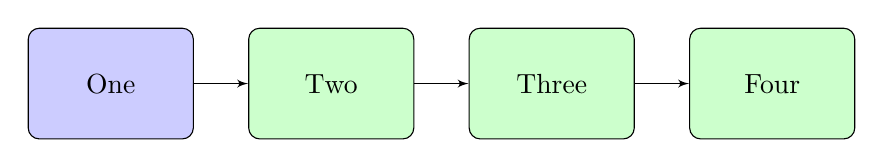
\begin{tikzpicture}[node distance = 2.8cm, auto]
      \node [block] (one) {One};
      \node [block, right of=one, fill=green!20] (two) {Two};
      \node [block, right of=two, fill=green!20] (three) {Three};
      \node [block, right of=three, fill=green!20] (four) {Four};
      % Draw edges
      \path [line] (one) -- (two);
      \path [line] (two) -- (three);
      \path [line] (three) -- (four);
    \end{tikzpicture}
  \end{frame}
  
  \begin{frame}
    \center{Questions?}
  \end{frame}
\end{document}